%
\documentclass[12pt]{article}

\usepackage{fullpage}
\usepackage{setspace}
\usepackage{endnotes}
%\usepackage{epsfig}
%\usepackage{psfrag}
\usepackage{amsmath}
\usepackage{amsfonts}
\usepackage{amssymb}
\usepackage{rotating}
\usepackage{dcolumn}
\usepackage{longtable}
\usepackage{microtype}
\usepackage{graphicx}
\usepackage{hyperref}
\usepackage[usenames,dvipsnames]{color}
%\usepackage{hypdvips}
\hypersetup{
 pdftitle={Compression and Conditional Effects}, % title
 pdfauthor={Redacted}, %Carlisle Rainey}, % author
 pdfkeywords={hypothesis testing}{interaction term}{product term}{interaction}{logit} {probit} {logisitic regression}
 pdfnewwindow=true, % links in new window
 colorlinks=true, % false: boxed links; true: colored links
 linkcolor=BrickRed, % color of internal links
 citecolor=BrickRed, % color of links to bibliography
 filecolor=BrickRed, % color of file links
 urlcolor=BrickRed % color of external links
}
\usepackage{url}
\usepackage{natbib}
%\bibpunct{(}{)}{,}{a}{}{;}
\usepackage{framed}
\usepackage{lipsum}
\usepackage[font=small,labelfont=sc]{caption}
 \usepackage{float}
\restylefloat{table}
\bibpunct{(}{)}{;}{a}{}{,}
\newtheorem{lemma}{Lemma}
\newtheorem{proposition}{Proposition}
\newtheorem{theorem}{Theorem}
\newtheorem{claim}{Claim}
\newenvironment{proof}[1][Proof]{\begin{trivlist}
\item[\hskip \labelsep {\bfseries #1}]}{\end{trivlist}}
\newenvironment{definition}[1][Definition]{\begin{trivlist}
\item[\hskip \labelsep {\bfseries #1}]}{\end{trivlist}}
\newenvironment{example}[1][Example]{\begin{trivlist}
\item[\hskip \labelsep {\bfseries #1}]}{\end{trivlist}}
\newenvironment{remark}[1][Remark]{\begin{trivlist}
\item[\hskip \labelsep {\bfseries #1}]}{\end{trivlist}}
%\newcommand{\qed}{\nobreak \ifvmode \relax \else
%      \ifdim\lastskip<1.5em \hskip-\lastskip
%      \hskip1.5em plus0em minus0.5em \fi \nobreak
%      \vrule height0.75em width0.5em depth0.25em\fi}
%      \setlength{\LTcapwidth}{5in}
%\def\p3s{\phantom{xxx}}

\usepackage{tgpagella}
\usepackage[T1]{fontenc}
%\usepackage[T1]{fontenc}
\usepackage[bitstream-charter]{mathdesign}


%Redefine the first level
\renewcommand{\theenumi}{\arabic{enumi}.}
\renewcommand{\labelenumi}{\theenumi}
%Redefine the second level
\renewcommand{\theenumii}{\alph{enumii}.}
\renewcommand{\labelenumii}{\theenumii}
%Redefine the third level
\renewcommand{\theenumiii}{\roman{enumiii}.}
\renewcommand{\labelenumiii}{\theenumiii}
%Redefine the fourth level
\renewcommand{\theenumiv}{\Alph{enumiv}.}
\renewcommand{\labelenumiv}{\theenumiv}


\parskip=0pt
\parindent=20pt
\usepackage{lscape}
\singlespace
\title{Compression and Conditional Effects}
%\author{Carlisle Rainey\thanks{Assistant Professor in the Department of Political Science at the University at Buffalo (SUNY)}}
\date{\today}
\usepackage[normalem]{ulem}

% Create footnote command so that my name
% has an asterisk rather than a one.
\long\def\symbolfootnote[#1]#2{\begingroup%
\def\thefootnote{\fnsymbol{footnote}}\footnote[#1]{#2}\endgroup}

\begin{document}
\begin{appendix}
\singlespace

\begin{center}
\LARGE{\textbf{Online Appendix for ``Compression and Conditional Effects''}}\vspace{4mm}
\end{center}
\section{Statistical Power}

Including a product term does reduce statistical power in tests of interaction using second-differences. If the researcher is correct and there is interaction due to compression (i.e., the logistic regression model is correct), then including a product term reduces the probability that the researcher will find a statistically significant interaction effect (i.e., the confidence interval for the second-difference does not contain zero). However, as I explain in the main text, statistical arguments proceed by fixing the size of the test at a suitably small value (usually 0.05) and then maximizing power. Maximizing power by increasing the size of one's test over-represents the evidence for one's hypotheses because readers expect the researcher to only accept their research hypothesis when the evidence overwhelmingly supports it. If power is maximized at the expense of size, then researchers accept their research hypothesis unless their is overwhelming evidence against it. Thus, I focus on the size of tests for interaction in the main text. Nonetheless, attentive researchers are conscious of the power of their tests, so I conduct a brief analysis here.

To estimate the power of tests for interaction with and without a product term, I simulate from the model (i.e., data-generating process) $\text{Pr}(Y) = \text{logit}^{-1}(\beta_xX - \beta_zZ)$, where $X$ is a continuous variable ranging from zero to one and $Z$ dichotomous variable that equals zero or one. I imagine that an analyst correctly suspects that $X$ has a positive effect on $\text{Pr}(Y)$, $Z$ has a negative effect on $\text{Pr}(Y)$, and that $X$ and $Z$ interact in influencing $\text{Pr}(Y)$ due to compression. That is, because the event is relatively common ($\text{Pr}(Y) > 0.5$) and $Z$ pushes $\text{Pr}(Y)$ even closer to zero, there is less room for $X$ to affect $\text{Pr}(Y)$. Therefore, the analyst expects that $X$ should have a smaller effect when $Z=1$. All three hypothesis are correct because logistic regression is the correct functional form. For varying values of $\beta_x$, $\beta_z$, and the sample size, I simulate 1,000 data sets and compute the proportion that have a statistically significant second-difference. Because $\beta_x$ and $\beta_z$ vary, the magnitude of this second-difference varies from trivially small (-0.02) to quite large (-0.21).

Because $X$ is approximately uniformly distributed from zero to one and $Z$ is dichotomous with half of the observations equal to one and the other half equal to zero, I test for interaction in each simulated data set by estimating a logistic regression model with and without a product term, calculating the second-difference as $X$ changes from 0.25 to 0.75 and $Z$ changes from zero to one. 

Notice that for trivial amounts of interaction (e.g., $\Delta\Delta = 0.07-0.09 = -0.02$), the model with a product term dramatically reduces the power of the test, especially for sample sizes around 1,000. However, for larger sample sizes and larger interaction effects, adding a product term to the model decreases the power of the test only slightly, while fixing the size of the test at a more typically value near 0.05 (see Figure 5 in the main text).

\begin{figure}[H]
\begin{center}
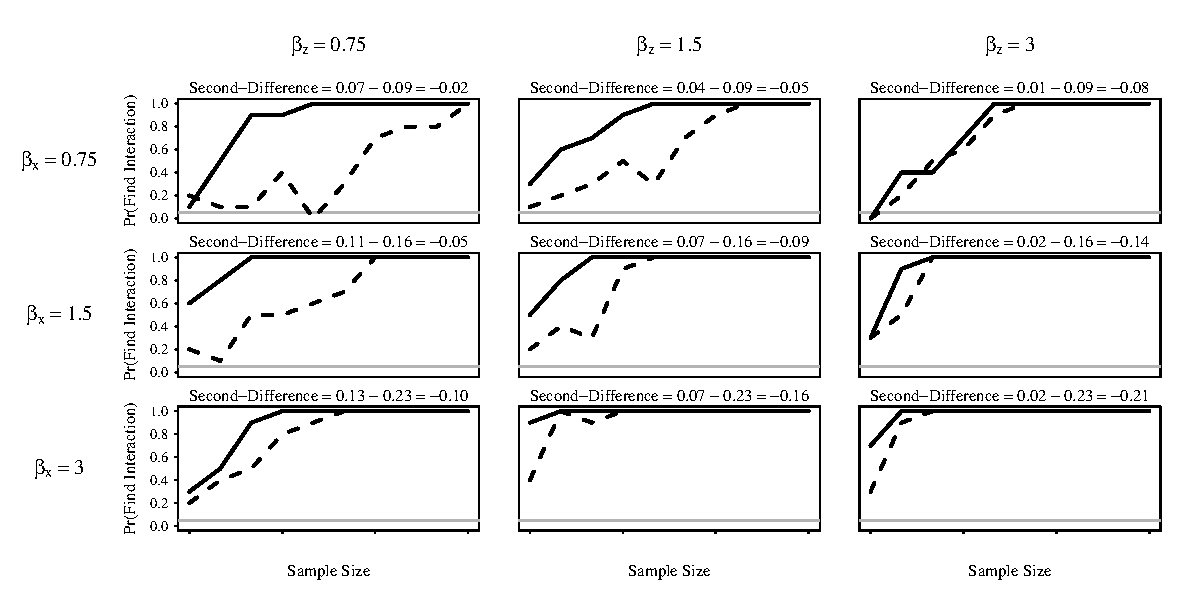
\includegraphics[scale = .8]{fig/fig-pwr.pdf}
\end{center}\caption{A figure showing the statistical power of models including a product term (dashed line) and excluding a product term (solid line) for detecting interaction. Notice that adding a product term decreases the power appreciably only for trivially small interaction effects (i.e., $\Delta\Delta = 0.07-0.09 = -0.02$).}\label{fig:pwr}
\end{figure}

\section{The Impact of Including an Unnecessary Product Term on Estimates of Effects of Other Variables}

One potential concern is that if the correct model is given by $\text{Pr}(Y) = \text{logit}^{-1}(\beta_{cons} + \beta_XX + \beta_ZZ + \beta_{W}W)$, then including an unnecessary interaction term $XZ$ will lead to biased estimates of the effect of other variables, such as $W$. Simulations show that this is not the case. No bias exists in estimates of the coefficient $\beta_W$ or the first difference $\text{Pr}(Y | W = w_{hi}) - \text{Pr}(Y | W = w_{lo})$. I only summarize a brief simulation here, but these result are identical for a range of other simulations I performed.

\begin{enumerate}
\item Set $N = 1000$. Setting the sample size to other values has no impact on the results.
\item Set $\beta_{cons} = 0$ and $\beta_X = \beta_Z = 1$. Setting these coefficients to other values has no impact on the results.
\item Draw $X$, $Z$, and $W$ from a $\text{Uniform}(0, 1)$ distribution to create the covariates. Using other distributions does not impact the results. Introducing correlations between the covariates does not impact the results.
\item As $\beta_W$ ranges from -1 to 1, do the following:
	\begin{enumerate}
	\item Compute $\pi = \text{Pr}(Y)$.
	\item To get an estimate of the expected value of the estimated effect of $W$, do the following 100,000 times.
		\begin{enumerate}
		\item Simulate $Y \sim \text{Bernoulli}(\pi)$.
		\item Estimate a logistic regression model with and without a product term.
		\item Store the coefficient for $W$.
		\item Calculate and store the first difference $\text{Pr}(Y | W = 0.75) - \text{Pr}(Y | W = 0.25)$.
		
		\end{enumerate}
	\item Calculate the mean of the estimated coefficients.
	\item Calculate the mean of the estimated first-differences
	\end{enumerate}
\end{enumerate}

As Figure \ref{fig:w-est} shows, the estimates of $\beta_W$ are not affected by the inclusions of an unnecessary product term. Particularly, there is no bias in either estimate. The mean estimates from the model with and without a product term entirely overlap with the true values. Figure \ref{fig:w-fd} shows that the same holds for the first difference.

\begin{figure}[H]
\begin{center}
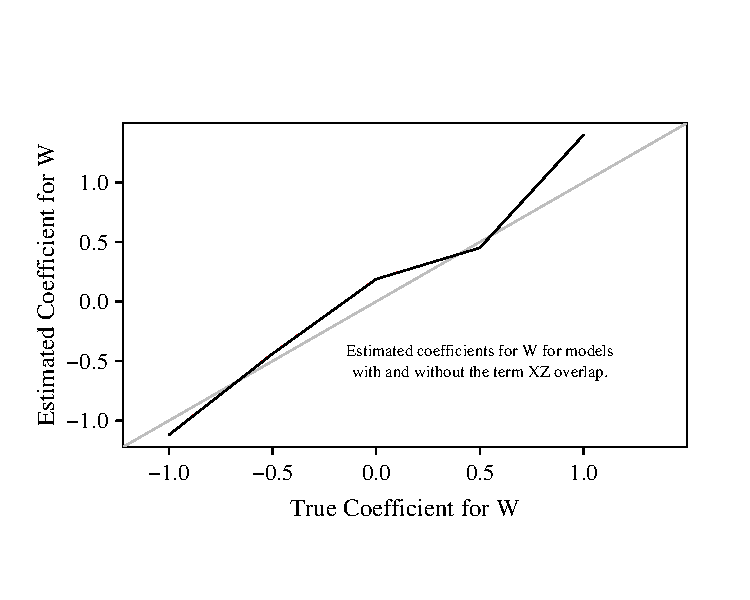
\includegraphics[scale = .8]{fig/fig-w-est.pdf}
\end{center}\caption{A figure showing the expected coefficient $E(\hat{\beta_W})$ as the true coefficient $\beta_W$ changes for the models with and without a product term. Note that the two overlap exactly, which means that including a product term does not bias the coefficients of other explanatory variables.}\label{fig:w-est}
\end{figure}

\begin{figure}[H]
\begin{center}
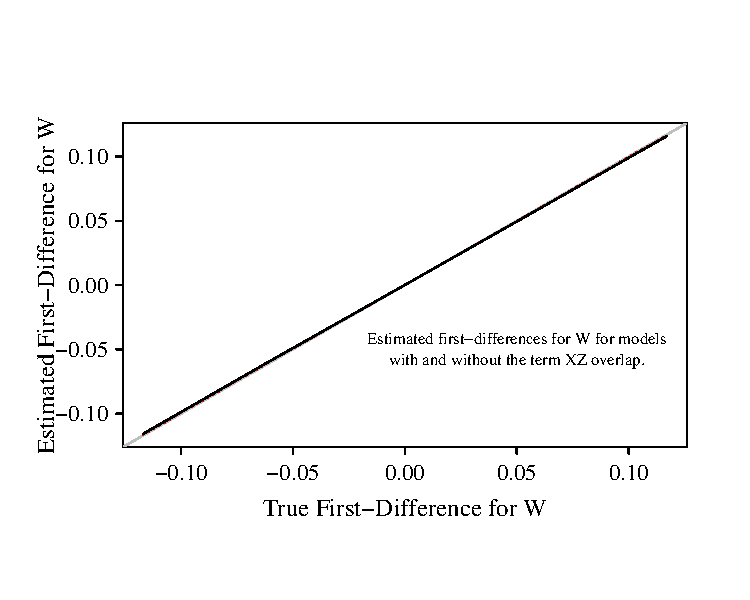
\includegraphics[scale = .8]{fig/fig-w-fd.pdf}
\end{center}\caption{A figure showing the expected estimate of the first-difference as the true first-difference changes for the models with and without a product term. Note that the two overlap exactly, which means that including a product term does not bias the first-differences of other explanatory variables.}\label{fig:w-fd}
\end{figure}

\section{Replication of the Fixed Process Simulation for Rare Events}

Particularly given the application of my ideas to the probability of conflict, one might wonder whether including a product term removes the bias as effectively when the event of interest is relatively rare. As a simple test case, I use the process $\text{Pr}(Y) = 0.04 + 0.04X - 0.02Z$, shown in Figure \ref{fig:relationships-fits-few1s} as a robustness check to the fixed process presented in Figure 3 of the main text. Notice, as before, that the model with a product term fits this non-interactive process surprisingly well and the model with no product term forces interaction into the estimates.

\begin{figure}[H]
\begin{center}
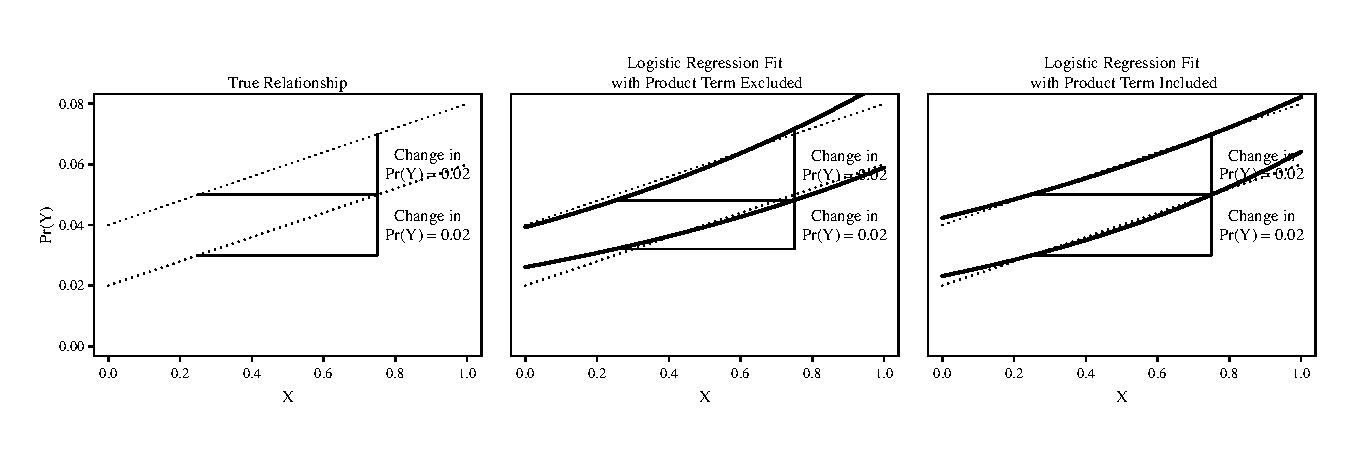
\includegraphics[width=\linewidth]{fig/fig-example-few1s.pdf}
%\vspace{-10mm}
\end{center}
\caption{This figure shows the true relationship in the ``rare events''  simulation study (dotted lines) as well as how logistic regression models with and without a product term fit the process (solid, bold lines). Notice that $X$ and $Z$ have small effects on $\text{Pr}(Y)$ and $\text{Pr}(Y)$ is always less than 0.1. In this case, excluding a product term forces the model to point toward interaction, despite the fact that the relationship is non-interactive. Including a product term allows the model to fit this non-interactive process surprisingly well. I use this process as a simple robustness check for the results presented in Figure \ref{fig:fixed}.}\label{fig:relationships-fits-few1s}
\end{figure}

Figure \ref{fig:fixed-few1s} presents the results from the fixed ``rare events'' process. For this rare events process, the product term does a much better job at removing the bias toward interaction than the process examined in the main text. Except for extremely large sample sizes near 100,000, the adding a product term removes nearly all of the bias and removes much of the bias even for the sample sizes near 100,000. The results suggest that the results presented in the main text represent a ``worst case'' scenario (that is what I had in mind when choosing the fixed process) and that the suggestion to include a product term applies to extremely rare (and, by symmetry, extremely common) as well as to events with probabilities closer to one-half.  

\begin{figure}[H]
\begin{center}
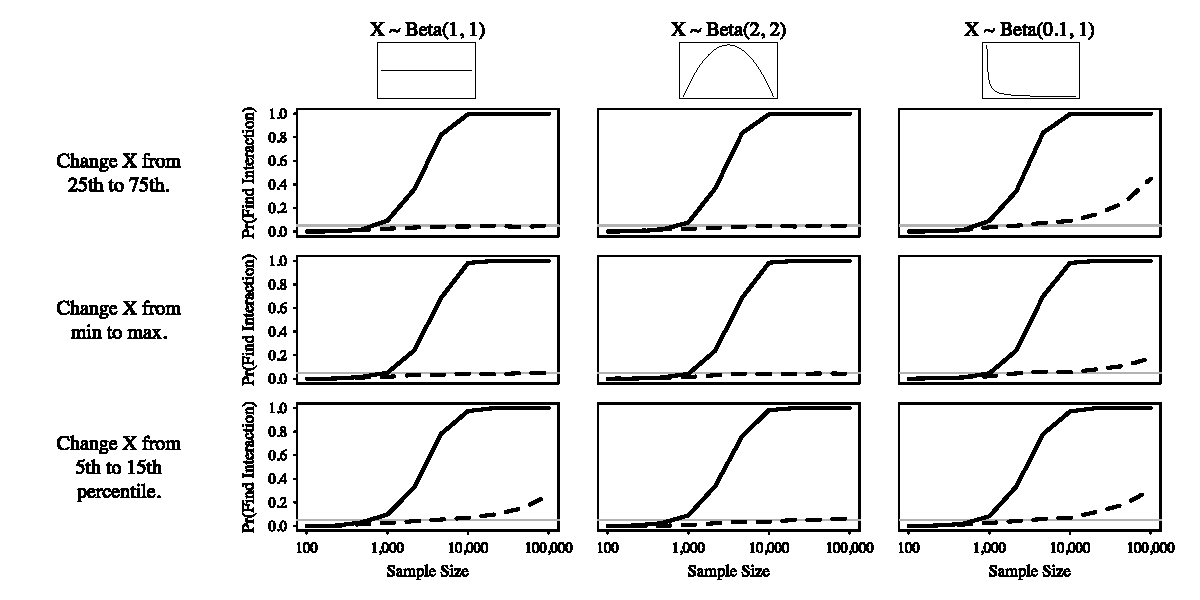
\includegraphics[scale = .8]{fig/fig-fixed-few1s.pdf}
\end{center}\caption{This figure shows the probability of concluding interaction when the true relationship is given by $\text{Pr}(Y) = 0.04 + 0.04X - 0.02Z$ (i.e., there is no interaction) using logistic regression models with and without a product term as the sample size, the distribution of $X$, and the change in $X$ considered in computing the second-difference varies. Notice that the model including a product term performs remarkably well, removing almost all of the bias except for extremely large samples. }\label{fig:fixed-few1s}
\end{figure}

\section{Generate a Random Analysis}

\begin{enumerate}
\item Choose a random relationship that is non-linear and non-interactive.
        \begin{enumerate}
        \item Draw $A$ and $B$ from a uniform distribution between 0.3 and 0.7.
        \item Draw $C$ from a uniform distribution between $A$ and $B$ if $A < B$ or between $B$ and $A$ if $B < A$.
        \item Draw $D$ from a uniform distribution between $A - 0.3$ and $A + 0.3$.
        \item Draw $E$ from a uniform distribution between 0 and $D$ if $D > 0$ or $D$ and 0 if $D < 0$.
        \item The true relationship is then given by $Pr(Y) = \beta_0 + \beta_1X + \beta_2Z + \beta_3X^2 + \beta_4Z^2$, where
                \begin{itemize}
                \item $\beta_1 = A$
                \item $\beta_2 = -3A - B + 4C$ 
                \item $\beta_3 = 4E - D$
                \item $\beta_4 = 2A + 2B - 4C$
                \item $\beta_5 = 2D - 4E$ 
                \end{itemize}
        \item Check the resulting relationship is monotonic as $X$ and $Z$ range from zero to one. If not, repeat until a monotonic relationship is obtained.
        \end{enumerate}
        Figure \ref{fig:choose-relationship} illustrates how this procedure works graphically and Figure    \ref{fig:relationship-sample} shows several randomly simulated relationships using this procedure.



        \item Choose a sample size by drawing from a Cauchy distribution, multiplying by 1,000, and rounding to the nearest whole number. The Cauchy distribution has very heavy tails so that most samples fall below 2,000, but very large samples (up to 100,000) occur as well. Table \ref{tab:n} provides the quantiles from this distribution.
        
        \item Choose the distribution of $X$ and $Z$. Perform the following to generate $X$ and $Z$.
                \begin{enumerate}
                \item Choose whether $X$ is binary or continuous. Set as binary with probability 0.5.
                \item If $X$ is continuous, choose the parameters of the Beta distribution from which it will be drawn from a uniform distribution from 0.7 to 3. Figure \ref{fig:distribution-sample}
                \item If $X$ is binary, choose the proportion of ones from a uniform distribution from 0.1 to 0.9.
                \item Repeat for $Z$.
                \end{enumerate}
                
        \item Choose the changes and $X$ and $Z$ used to test for interaction.
                \begin{enumerate}
                \item If $X$ is binary, set $\langle x_{lo}, x_{hi} \rangle$ to $\langle 0, 1 \rangle$.
                \item If $X$ is continuous, then draw and sort two values from a uniform distribution from zero to one. Set these sorted draws as $\langle x_{lo}, x_{hi} \rangle$.
                \item Repeat for $Z$.
                \end{enumerate}
\end{enumerate}

\begin{table}[h]
\begin{center}
\begin{tabular}{|cc|}
\hline
Percentile & Sample Size \\ 
\hline
0\% & 500 \\ 
10\% & 646 \\ 
20\% & 815 \\ 
30\% & 1,019 \\ 
40\% & 1,276 \\ 
50\% & 1,614 \\ 
60\% & 2,105 \\ 
70\% & 2,896 \\ 
80\% & 4,427 \\ 
90\% & 8,896 \\ 
100\% & 100,000 \\ 
\hline
\end{tabular}\caption{The distribution of sample sizes I used to simulate analyses.}\label{tab:n}
\end{center}
\end{table}     

        \begin{figure}[h]
        \begin{center}
        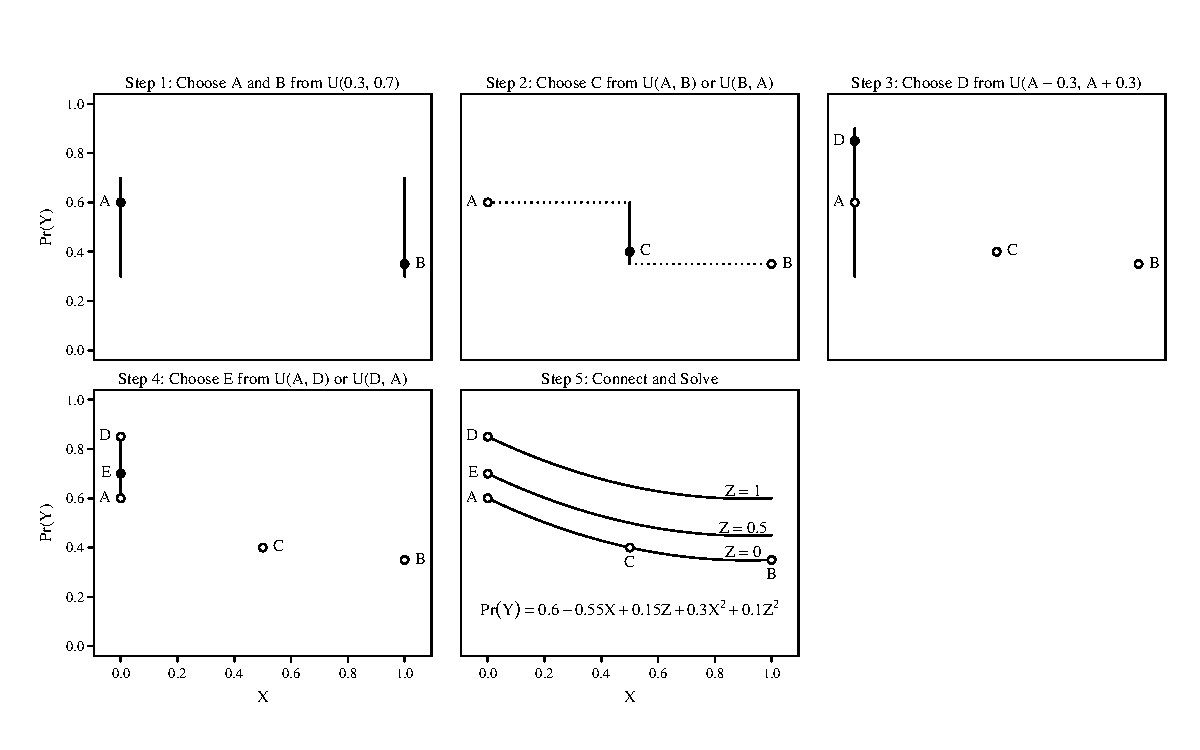
\includegraphics[width = \linewidth]{fig/fig-choose-relationship.pdf}
        \end{center}\caption{This figure graphically illustrates how I generate random relationships that are non-interactive and non-linear using the procedure describe in Step 1.}\label{fig:choose-relationship}
        \end{figure}
        
 
              \begin{figure}[h]
        \begin{center}
        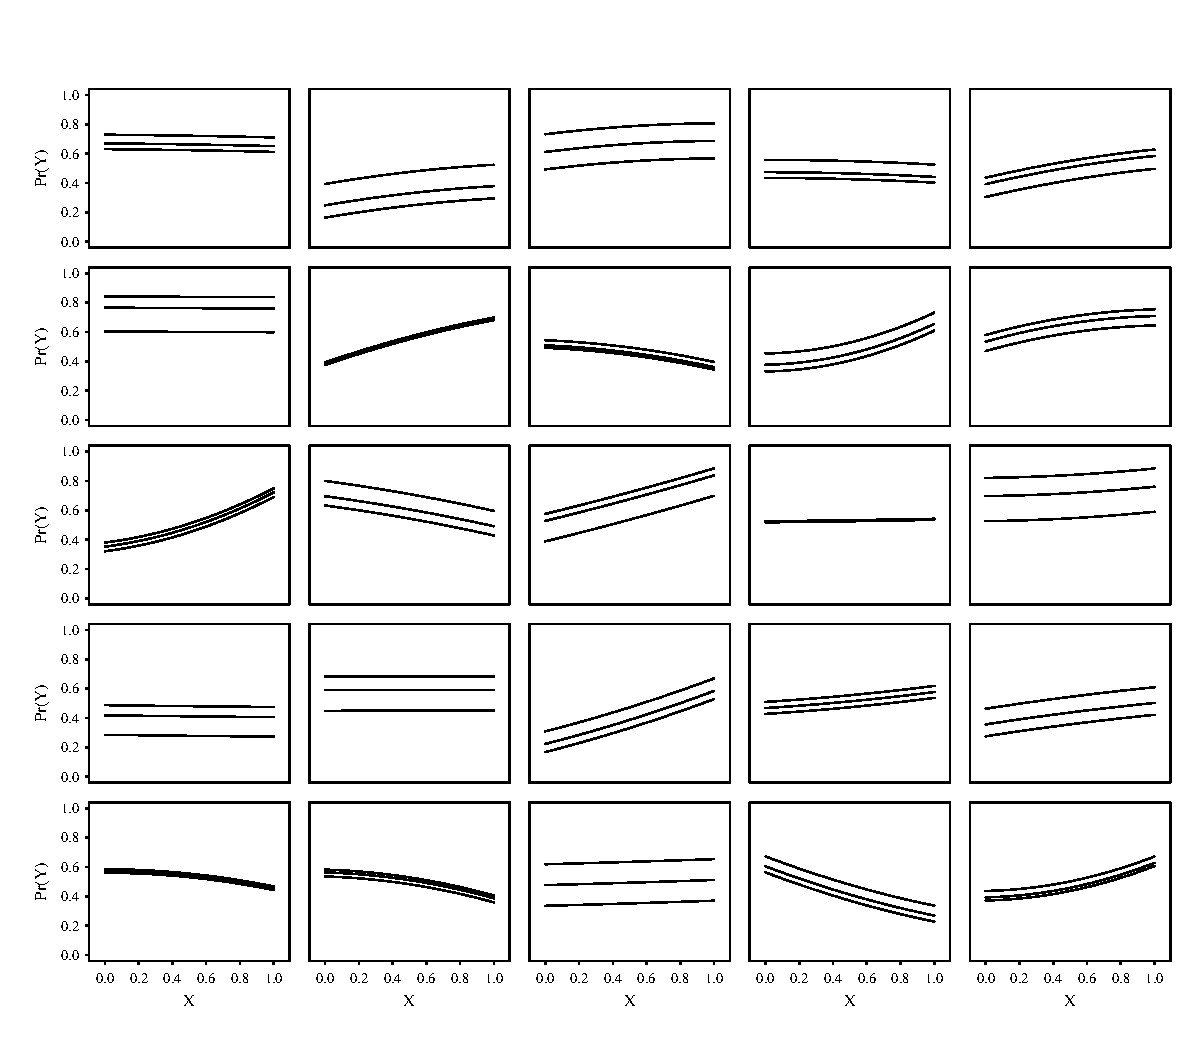
\includegraphics[width = \linewidth]{fig/fig-relationship-sample.pdf}
        \end{center}\caption{This figure shows several relationships randomly generated using the steps described in Figure \ref{fig:choose-relationship} and Step 1 of the algorithm above. The three lines represent the relationship between $X$ and $\text{Pr}(Y)$ when $Z$ equals zero, one-half, and one, respectively. Due to the assumption of monotonicity described in Step 1(f), the line for which $Z = 0.5$ must fall between the other two.}\label{fig:relationship-sample}
        \end{figure}
        
                                \begin{figure}[h]
        \begin{center}
        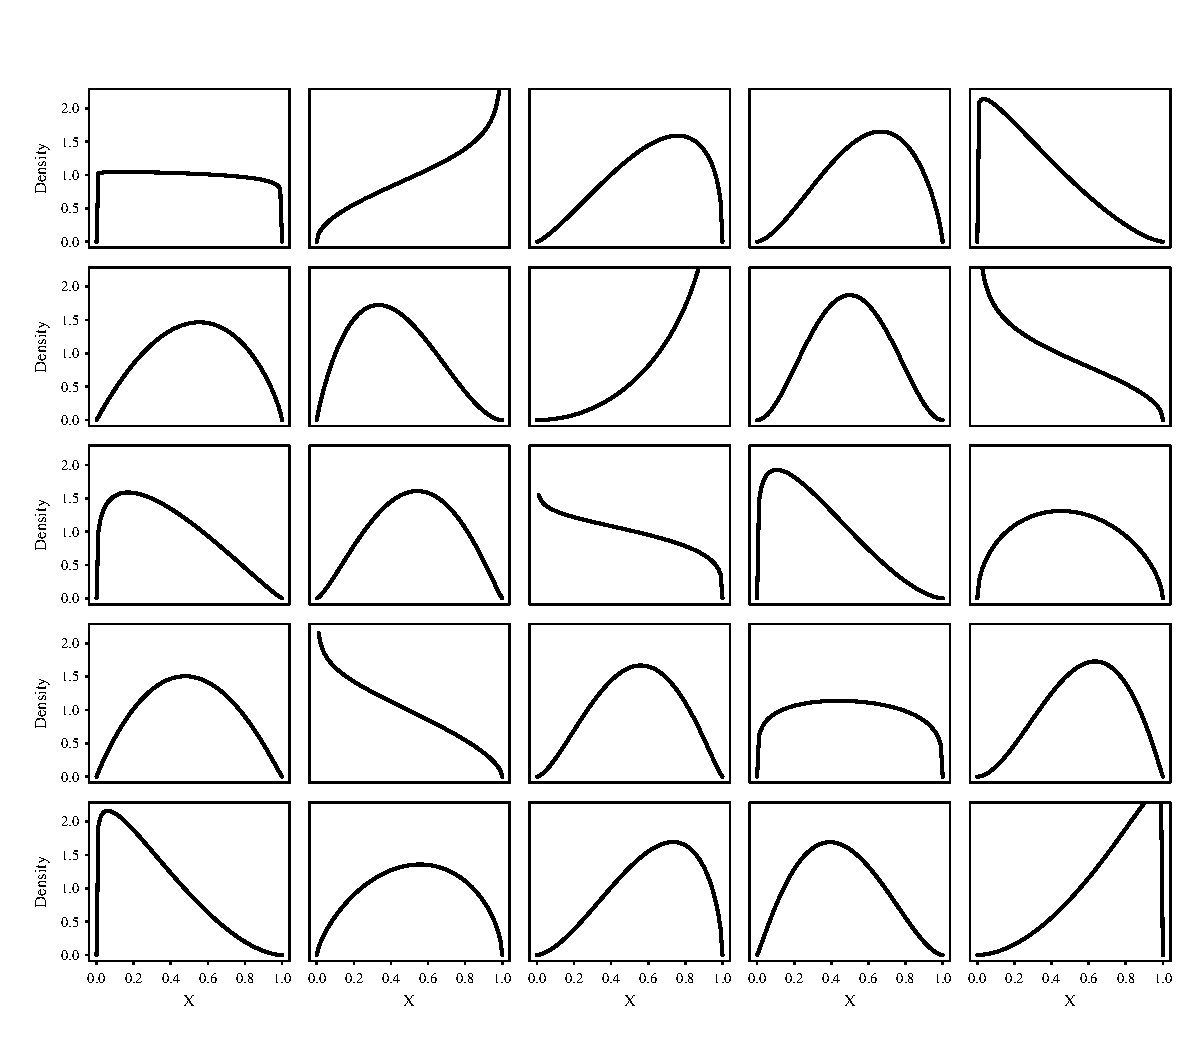
\includegraphics[width = \linewidth]{fig/fig-distribution-sample.pdf}
        \end{center}\caption{This figure shows several possible continuous distributions of $X$ (or $Z$) randomly generated using Step 3(b). }\label{fig:distribution-sample}
        \end{figure}
        
\clearpage        
        
\section{Model Estimates}

As \cite{BramborClarkGolder2006} and \cite{BerryDeMerittEsarey2010} explain, examining tables of coefficients is not always helpful for evaluating interactive hypotheses with logistic regression models. In the main text I present plots of predicted probabilities (Figure \ref{fig:pr-distance}), first-differences (Figures \ref{fig:fd-distance} and \ref{fig:fd-democracy}), and second-differences (Figure \ref{fig:sd-distance}). Table \ref{tab:coefficients} presents the coefficients and standard errors for reference.

Relying on the model with no product term, we can immediately evaluate the evidence for the Democracy and Distance Hypotheses by looking at the coefficients for Lower Democracy and log(Distance). We can see that both of these estimates are negative (as expected) and statistically significant. Further, based on this model, we can already conclude that the negative effect of log(Distance) is smaller in more democratic dyads since (1) both coefficients are negative and (2) conflict is relatively rare (i.e., the probability of conflict falls well below 0.5).

\begin{table}[H]
\begin{center}
\begin{footnotesize}
\begin{tabular}{l c c }
\hline
                                       & No Product Term & Product Term \\
\hline
Lower Democracy                        & $-0.091^{***}$ & $-0.121^{***}$ \\
                                       & $(0.005)$      & $(0.025)$      \\
Log(Distance)                          & $-0.306^{***}$ & $-0.285^{***}$ \\
                                       & $(0.026)$      & $(0.031)$      \\
Lower Democracy $\times$ Log(Distance) &                & $0.004$        \\
                                       &                & $(0.004)$      \\
Allies                                 & $-0.694^{***}$ & $-0.697^{***}$ \\
                                       & $(0.063)$      & $(0.063)$      \\
Power Ratio                            & $-0.264^{***}$ & $-0.262^{***}$ \\
                                       & $(0.019)$      & $(0.019)$      \\
Noncontiguity                          & $-0.980^{***}$ & $-0.982^{***}$ \\
                                       & $(0.073)$      & $(0.073)$      \\
Only Minor Powers                      & $-0.467^{***}$ & $-0.475^{***}$ \\
                                       & $(0.070)$      & $(0.071)$      \\
Constant                               & $-1.222^{***}$ & $-1.370^{***}$ \\
                                       & $(0.202)$      & $(0.237)$      \\
\hline
AIC                                    & 13,520      & 13,520      \\
BIC                                    & 13,580      & 13,589      \\
Num. obs.                              & 39,996          & 39,996          \\
\hline
\multicolumn{3}{l}{\scriptsize{\textsuperscript{***}$p<0.001$, 
  \textsuperscript{**}$p<0.01$, 
  \textsuperscript{*}$p<0.05$}}
\end{tabular}
\end{footnotesize}
\caption{Logistic regression models of the probability of conflict in each dyad-year. The model in the left column excludes the product term, as suggested by \cite{BerryDeMerittEsarey2010}. The model in the right column includes a product term. Notice that although the product term is not statistically significant and the BIC for this model is higher (suggesting a worse fit), including this product term allows a more compelling test of the Interaction Hypothesis.}
\label{tab:coefficients}
\end{center}
\end{table}

\singlespace
\bibliographystyle{apsr_fs}
%\bibliography{/Users/rcrainey/Dropbox/Bibliography/bibliography.bib}
\bibliography{bibliography.bib}

\end{appendix}
\end{document}



